%% Template for MLP Coursework 2 / 13 November 2023

%% Based on  LaTeX template for ICML 2017 - example_paper.tex at 
%%  https://2017.icml.cc/Conferences/2017/StyleAuthorInstructions

\documentclass{article}
\usepackage[T1]{fontenc}
\usepackage{amssymb,amsmath}
\usepackage{txfonts}
\usepackage{microtype}

% For figures
\usepackage{graphicx}
\usepackage{subcaption} 

% For citations
\usepackage{natbib}

% For algorithms
\usepackage{algorithm}
\usepackage{algorithmic}

% the hyperref package is used to produce hyperlinks in the
% resulting PDF.  If this breaks your system, please commend out the
% following usepackage line and replace \usepackage{mlp2017} with
% \usepackage[nohyperref]{mlp2017} below.
\usepackage{hyperref}
\usepackage{url}
\urlstyle{same}

\usepackage{color}
\usepackage{booktabs} % To thicken table lines
\usepackage{multirow} % Multirow cells in table
\usepackage{soul}
\usepackage{bm}

% Packages hyperref and algorithmic misbehave sometimes.  We can fix
% this with the following command.
\newcommand{\theHalgorithm}{\arabic{algorithm}}


% Set up MLP coursework style (based on ICML style)
\usepackage{mlp2022}
\mlptitlerunning{MLP Coursework 1 (\studentNumber)}
\bibliographystyle{icml2017}


\DeclareMathOperator{\softmax}{softmax}
\DeclareMathOperator{\sigmoid}{sigmoid}
\DeclareMathOperator{\sgn}{sgn}
\DeclareMathOperator{\relu}{relu}
\DeclareMathOperator{\lrelu}{lrelu}
\DeclareMathOperator{\elu}{elu}
\DeclareMathOperator{\selu}{selu}
\DeclareMathOperator{\maxout}{maxout}



\definecolor{red}{rgb}{0.95,0.4,0.4}
\definecolor{blue}{rgb}{0.4,0.4,0.95}
\definecolor{orange}{rgb}{1, 0.65, 0}

\newcommand{\youranswer}[1]{{\color{red} \bf[#1]}} %your answer: 


%% START of YOUR ANSWERS
%% REPLACE sXXXXXXX with your student number
\def\studentNumber{s2617343}


%% START of YOUR ANSWERS
%% Add answers to the questions below, by replacing the text inside the brackets {} for \youranswer{ "Text to be replaced with your answer." }. 
%
% Do not delete the commands for adding figures and tables. Instead fill in the missing values with your experiment results, and replace the images with your own respective figures.
%
% You can generally delete the placeholder text, such as for example the text "Question Figure 3 - Replace the images ..." 
%
% There are 5 TEXT QUESTIONS. Replace the text inside the brackets of the command \youranswer with your answer to the question.
%
% There are also 3 "questions" to replace some placeholder FIGURES with your own, and 1 "question" asking you to fill in the missing entries in the TABLE provided. 
%
% NOTE! that questions are ordered by the order of appearance of their answers in the text, and not necessarily by the order you should tackle them. You should attempt to fill in the TABLE and FIGURES before discussing the results presented there. 
%
% NOTE! If for some reason you do not manage to produce results for some FIGURES and the TABLE, then you can get partial marks by discussing your expectations of the results in the relevant TEXT QUESTIONS. The TABLE specifically has enough information in it already for you to draw meaningful conclusions.
%
% Please refer to the coursework specification for more details.


%% - - - - - - - - - - - - TEXT QUESTIONS - - - - - - - - - - - - 

%% Question 1 - Use Figures 1, 2, and 3 to identify the Vanishing Gradient Problem (which of these model suffers from it, and what are the consequences depicted?).

% The average length for an answer to this question is approximately 1/5 of the columns in a 2-column page
\newcommand{\questionOne} {
\youranswer{By comparing Figure~\ref{fig:grad_flow_08} and Figure~\ref{fig:avg_grad_flow_38}, it is clear that VGG08 maintains significantly larger gradients across all layers (e.g., 0.025 at the bottom and 0.05-0.2 at the top). In contrast, VGG38 exhibits almost zero gradients beyond the bottom regression layer (~0.00035) and dimensionality reduction block (~0.000025), indicating a severe vanishing gradient problem.

This occurs because gradients diminish exponentially during backpropagation due to the chain rule, leaving top-layer gradients effectively zero. As a result, parameter updates fail in most layers, halting learning. This is reflected in Figure~\ref{fig:curves}, where VGG38's accuracy remains at 0 throughout training, despite increasing epochs.
}
}

%% Question 2 - Consider these results (including Figure 1 from \cite{he2016deep}). Discuss the relation between network capacity and overfitting, and whether, and how, this is reflected on these results. What other factors may have lead to this difference in performance?

% The average length for an answer to this question is
% approximately 1/5 of the columns in a 2-column page
\newcommand{\questionTwo} {
\youranswer{Generally, as network capacity increases, the model’s expressive power is expected to improve. However, larger-capacity models can suffer from overfitting, where the model learns data noise instead of general patterns. Additionally, differences in performance between networks of varying capacities may result from the vanishing gradient problem, as shown in Figure~\ref{fig:curves}. Larger models also introduce more parameters, requiring higher computational resources and leading to slower convergence.

In Figure 1 from \cite{he2016deep}, the 56-layer network underperforms compared to the 20-layer network, highlighting the model degradation problem. This issue is not necessarily due to overfitting but could stem from optimization challenges, such as insufficient convergence speed or difficulty propagating gradients effectively in deeper networks.}
}

%% Question 3 - In this coursework, we didn't incorporate residual connections to the downsampling layers. Explain and justify what would need to be changed in order to add residual connections to the downsampling layers. Give and explain 2 ways of incorporating these changes and discuss pros and cons of each.
\newcommand{\questionThree} {
\youranswer{Adding residual connections to a network requires that the input and output of the block have exactly the same shape; otherwise, additive residual connections cannot be performed. However, downsampling layers typically alter the output shape, making it incompatible with direct addition of residual connections.

We propose two solutions to address this issue. The first solution is to add a 1x1 convolution block to the residual connection to adjust the input shape, ensuring it matches the output shape. The advantage of this approach is its high flexibility, as the 1x1 convolution allows learning additional parameters to better retain input information. However, this method increases computational cost and model complexity.

The second solution is to add the same downsampling layer (e.g. average pooling) to the residual connection. This also aligns the input and output shapes, allowing residual addition. The advantage of this method is its simplicity and lack of additional computational overhead. However, the downside is that downsampling layers may lose important input information during the process.

Both methods enable residual connections in downsampling layers, but the choice depends on the specific requirements.}
}

%% Question 4 - Present and discuss the experiment results (all of the results and not just the ones you had to fill in) in Table 1 and Figures 4 and 5 (you may use any of the other Figures if you think they are relevant to your analysis). You will have to determine what data are relevant to the discussion, and what information can be extracted from it. Also, discuss what further experiments you would have ran on any combination of VGG08, VGG38, BN, RC in order to
% \begin{itemize}
%     \item Improve performance of the model trained (explain why you expect your suggested experiments will help with this).
%     \item Learn more about the behaviour of BN and RC (explain what you are trying to learn and how).
% \end{itemize}

% The average length for an answer to this question is approximately 1 of the columns in a 2-column page
\newcommand{\questionFour} {
\youranswer{From our experimental results, Batch Normalization (BN) and Residual Connections (RC) effectively alleviate the vanishing gradient problem and improve model performance. The specific effects can be observed in Table~\ref{tab:CIFAR_results}. First, by comparing VGG08 and VGG38, it is evident that deeper networks with larger capacity are more susceptible to the vanishing gradient problem. By adding BN and RC layers to VGG38, we observe a significant improvement in performance, as these methods successfully mitigate the gradient vanishing issue. Comparing the validation accuracy (val acc), we may infer that RC has a slightly greater impact than BN. 

Furthermore, by varying the learning rate, we found that the BN layer is less sensitive to learning rate changes, while the RC layer is more sensitive. This implies that adjusting the learning rate can further optimize networks with RC layers. Figure 6 from \cite{he2016deep} also demonstrates that BN effectively addresses gradient vanishing on its own, but the introduction of RC layers further enhances convergence on top of BN. Based on these experiments, we conclude that the best model configuration is VGG38 with BN and RC layers (learning rate of 1e-2). By analyzing its training curve (Figure~\ref{fig:training_curves_bestModel}) and gradient flow (Figure~\ref{fig:avg_grad_flow_bestModel}), we observe that this model mitigates the vanishing gradient problem well and achieves the highest validation accuracy of 59.92. However, there are signs of slight overfitting, and the validation curve exhibits greater volatility, possibly due to the model's sensitivity to the learning rate.

To further improve model performance, I suggest the following experimental designs:
1. Add BN and RC layers to VGG08 to test whether their benefits extend to shallower networks. Given their success with VGG38, this could reveal whether these methods are universally applicable or more effective in deeper networks.
2. Incorporate appropriate regularization methods, such as Dropout or L1 norm penalties, to mitigate the overfitting observed in the current best-performing model.

To further investigate the effects of BN and RC layers, I propose the following experimental directions:
1. Evaluate whether the effects of BN and RC remain consistent across networks of varying depths, such as VGG08 and VGG38.
2. Explore the effect of learning rates on networks with only RC layers, given our observation that learning rate has minimal impact on networks with only BN layers.
3. Examine whether BN and RC independently enhance model performance or if there is an interaction between the two methods that amplifies their effectiveness.

These additional experiments will provide deeper insights into the behavior and benefits of BN and RC layers across different set up.}
}


%% Question 5 - Briefly draw your conclusions based on the results from the previous sections (what are the take-away messages?) and conclude your report with a recommendation for future work. 

% Good recommendations for future work also draw on the broader literature (the papers already referenced are good starting points). Great recommendations for future work are not just incremental (an example of an incremental suggestion would be: ``we could also train with different learning rates'') but instead also identify meaningful questions or, in other words, questions with answers that might be somewhat more generally applicable. 

% For example, \citep{huang2017densely} end with \begin{quote}``Because of their compact internal representations and reduced feature redundancy, DenseNets may be good feature extractors for various computer vision tasks that build on convolutional features, e.g.,  [4,5].''\end{quote} 

% while \cite{bengio1993problem} state in their conclusions that \begin{quote}``There remains theoretical questions to be considered,  such as whether the problem with simple gradient descent  discussed in this paper would be observed with  chaotic attractors that are not  hyperbolic.''\\\end{quote}

% The length of this question description is indicative of the average length of a conclusion section
\newcommand{\questionFive} {
\youranswer{In this paper, we primarily investigated the vanishing gradient problem in deep networks. We found that simply increasing the number of layers in a model can lead to the gradient failing to propagate effectively to the upper layers, thereby hindering parameter updates. To address this issue, we explored two solutions: Batch Normalization (BN) and Residual Connections (RC). Both methods were applied to the original VGG38 model, and extensive experimental results demonstrated that these methods effectively mitigate the vanishing gradient problem. Additionally, our results highlight the potential for further experiments to explore the specific effects of BN and RC layers on model performance. 

Given that BN and RC layers have proven effective in addressing the vanishing gradient problem, we also observed that ResNet architectures fundamentally resolve the issue of network depth. By incorporating residual connections, ResNet enables deeper networks to maintain gradient flow. However, as noted in \cite{he2016deep}, the performance of very deep ResNets does not always surpass that of shallower ResNets. This suggests that network depth is no longer the primary limitation, and future research should instead focus on improving network optimization. Specifically, we recommend exploring methods to accelerate the convergence of large-capacity networks and address overfitting challenges.

In conclusion, while significant progress has been made in mitigating gradient-related issues, optimizing deeper networks remains an open problem. Future work could include designing better regularization techniques, exploring adaptive learning rate strategies for large-scale models, and investigating alternative architectures that balance depth, capacity, and generalization ability.}
}


%% - - - - - - - - - - - - FIGURES - - - - - - - - - - - - 

%% Question Figure 3 - Replace this image with a figure depicting the average gradient across layers, for the VGG38 model.

% \textit{(The provided figure is correct, and can be used in your analysis. It is partially obscured so you can get credit for producing your own copy).}
\newcommand{\questionFigureThree} {
\youranswer{
    Question Figure~\ref{fig:avg_grad_flow_38}
%
\begin{figure}[t]
    \centering
    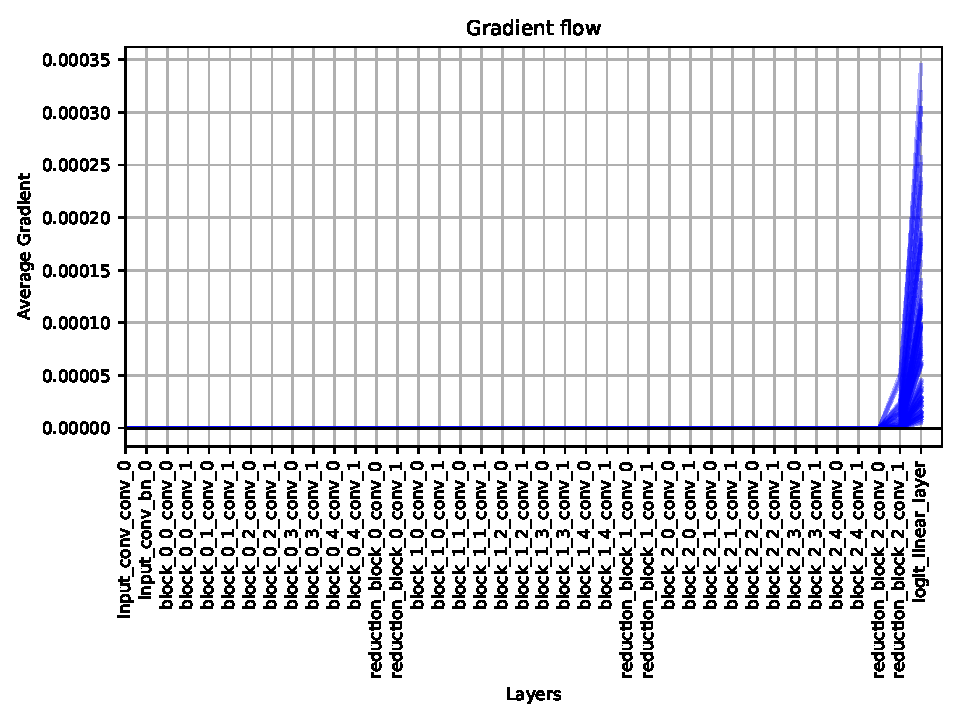
\includegraphics[width=\linewidth]{figures/myanswer_VGG_38.pdf} % figures/gradplot_38_watermarked.pdf
    \caption{Gradient Flow on VGG38}
    \label{fig:avg_grad_flow_38}
\end{figure}
}
}

%% Question Figure 4 - Replace this image with a figure depicting the training curves for the model with the best performance \textit{across experiments you have available (you don't need to run the experiments for the models we already give you results for)}. Edit the caption so that it clearly identifies the model and what is depicted.
\newcommand{\questionFigureFour} {
\youranswer{
    Question Figure~\ref{fig:training_curves_bestModel}
%
\begin{figure}[t]
    \centering
    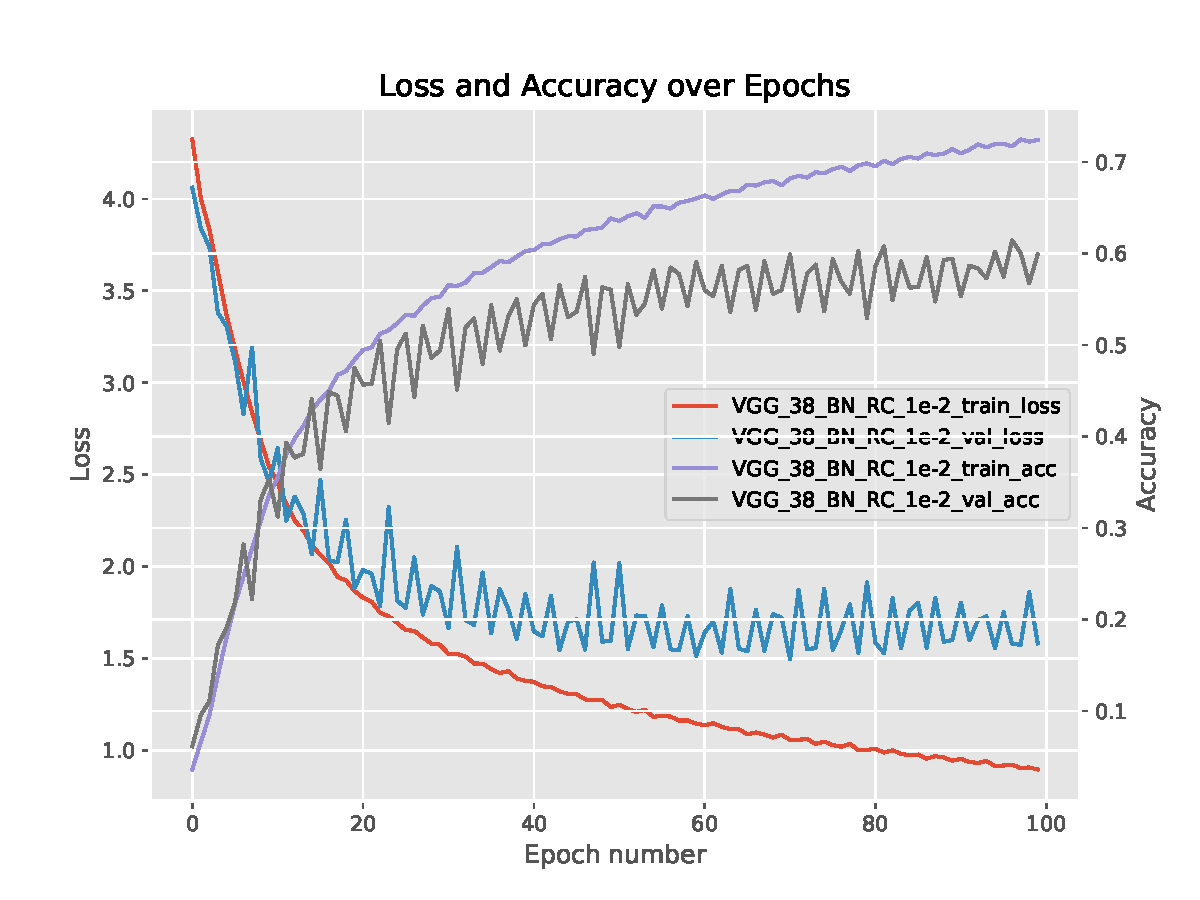
\includegraphics[width=\linewidth]{figures/myanswer_VGG_38_BN_RC_training_curve_big_figure.pdf}
    \caption{Training curves for VGG38 with Batch Normalisation and Residual Connection (Learning Rate 1e-2) in terms of cross-entropy error (left Y-axis) and classification accuracy (right Y-axis)}
    \label{fig:training_curves_bestModel}
\end{figure}
}
}

%% Question Figure 5 - Replace this image with a figure depicting the average gradient across layers, for the model with the best performance \textit{across experiments you have available (you don't need to run the experiments for the models we already give you results for)}. Edit the caption so that it clearly identifies the model and what is depicted.
\newcommand{\questionFigureFive} {
\youranswer{
    Question Figure~\ref{fig:avg_grad_flow_bestModel}
%
\begin{figure}[t]
    \centering
    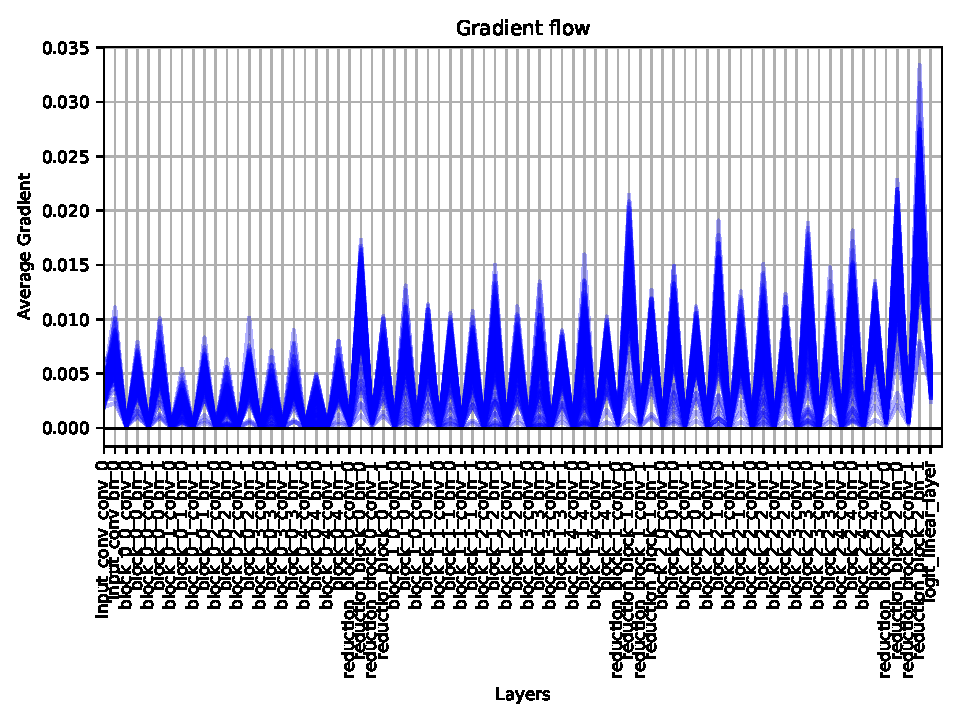
\includegraphics[width=\linewidth]{figures/myanswer_VGG_38_BN_RC_gradient_flow.pdf}
    \caption{Gradient Flow on VGG38 with Batch Normalisation and Residual Connection (Learning Rate 1e-2)}
    \label{fig:avg_grad_flow_bestModel}
\end{figure}
}
}

%% - - - - - - - - - - - - TABLES - - - - - - - - - - - - 

%% Question Table 1 - Fill in Table 1 with the results from your experiments on 
% \begin{enumerate}
%     \item \textit{VGG38 BN (LR 1e-3)}, and 
%     \item \textit{VGG38 BN + RC (LR 1e-2)}.
% \end{enumerate}
\newcommand{\questionTableOne} {
\youranswer{
    Question Table~\ref{tab:CIFAR_results}
%
\begin{table*}[t]
    \centering
    \begin{tabular}{lr|ccccc}
    \toprule
        Model                   & LR   & \# Params & Train loss & Train acc & Val loss & Val acc \\
    \midrule
        VGG08                   & 1e-3 & 60 K      &  1.74      & 51.59     & 1.95     & 46.84 \\
        VGG38                   & 1e-3 & 336 K     &  4.61      & 00.01     & 4.61     & 00.01 \\
        VGG38 BN                & 1e-3 & 339 K     &  1.70      & 52.16     & 1.84     & 48.08 \\
        VGG38 RC                & 1e-3 & 336 K     &  1.33      & 61.52     & 1.84     & 52.32 \\
        VGG38 BN + RC           & 1e-3 & 339 K     &  1.26      & 62.99     & 1.73     & 53.76 \\
        VGG38 BN                & 1e-2 & 339 K     &  1.70      & 52.28     & 1.99     & 46.72 \\
        VGG38 BN + RC           & 1e-2 & 339 K     &  0.90      & 72.43     & 1.58     & 59.92 \\
    \bottomrule
    \end{tabular}
    \caption{Experiment results (number of model parameters, Training and Validation loss and accuracy) for different combinations of VGG08, VGG38, Batch Normalisation (BN), and Residual Connections (RC), LR is learning rate.}
    \label{tab:CIFAR_results}
\end{table*} 
}
}

%% END of YOUR ANSWERS

%% END of YOUR ANSWERS



%% Do not change anything in this file. Add your answers to mlp-cw1-questions.tex



\begin{document} 

\twocolumn[
\mlptitle{MLP Coursework 2}
\centerline{\studentNumber}
\vskip 7mm
]

\begin{abstract} 
Deep neural networks have become the state-of-the-art 
in many standard computer vision problems thanks to their powerful
representations and availability of large labeled datasets.
While very deep networks allow for learning more levels of abstractions in their layers from the data, training these models successfully is a challenging task due to problematic gradient flow through the layers, known as vanishing/exploding gradient problem.
In this report, we first analyze this problem in VGG models with 8 and 38 hidden layers on the CIFAR100 image dataset, by monitoring the gradient flow during training. 
We explore known solutions to this problem including batch normalization or residual connections, and explain their theory and implementation details. 
Our experiments show that batch normalization and residual connections effectively address the aforementioned problem and hence enable a deeper model to outperform shallower ones in the same experimental setup.
\end{abstract} 

\section{Introduction}
\label{sec:intro}
Despite the remarkable progress of modern convolutional neural networks (CNNs) in image classification problems~\cite{simonyan2014very, he2016deep}, training very deep networks is a challenging procedure.
One of the major problems is the Vanishing Gradient Problem (VGP), a phenomenon where the gradients of the error function with respect to network weights shrink to zero, as they backpropagate to earlier layers, hence preventing effective weight updates. 
This phenomenon is prevalent and has been extensively studied in various deep neural networks including feedforward  networks~\cite{glorot2010understanding},  RNNs~\cite{bengio1993problem}, and CNNs~\cite{he2016deep}. 
Multiple solutions have been proposed to mitigate this problem by using weight initialization strategies~\cite{glorot2010understanding},
activation functions~\cite{glorot2010understanding}, input normalization~\cite{bishop1995neural},
batch normalization~\cite{ioffe2015batch}, and shortcut connections \cite{he2016deep, huang2017densely}.

This report focuses on diagnosing the VGP occurring in the VGG38 model\footnote{VGG stands for the Visual Geometry Group in the University of Oxford.} and addressing it by implementing two standard solutions.
In particular, we first study a ``broken'' network in terms of its gradient flow, L1 norm of gradients with respect to its weights for each layer and contrast it to ones in the healthy and shallower VGG08 to pinpoint the problem.
Next, we review two standard solutions for this problem,  batch normalization (BN)~\cite{ioffe2015batch} and residual connections (RC)~\cite{he2016deep} in detail and discuss how they can address the gradient problem.
We first incorporate batch normalization (denoted as VGG38+BN), residual connections (denoted as VGG38+RC),  and their combination (denoted as VGG38+BN+RC) to the given VGG38 architecture.
We train the resulting three configurations, and VGG08 and VGG38 models on CIFAR100 (pronounced as `see far 100' ) dataset and present the results.
The results show that though separate use of BN and RC does mitigate the vanishing/exploding gradient problem, therefore enabling effective training of the VGG38 model, the best results are obtained by combining both BN and RC.

%


\section{Identifying training problems of a deep CNN}
\label{sec:task1}

\begin{figure}[t]
    \begin{subfigure}{\linewidth}
        \centering
        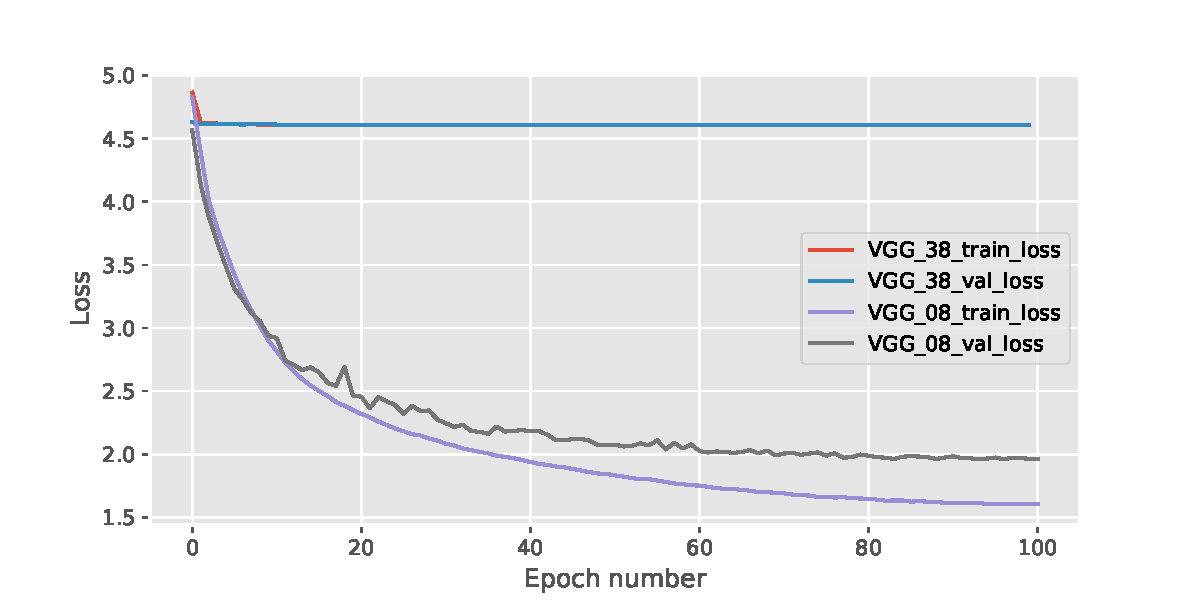
\includegraphics[width=\linewidth]{figures/loss_plot.pdf}
        \caption{Cross entropy error per epoch}
        \label{fig:loss_curves}
    \end{subfigure}

    \begin{subfigure}{\linewidth}
        \centering
        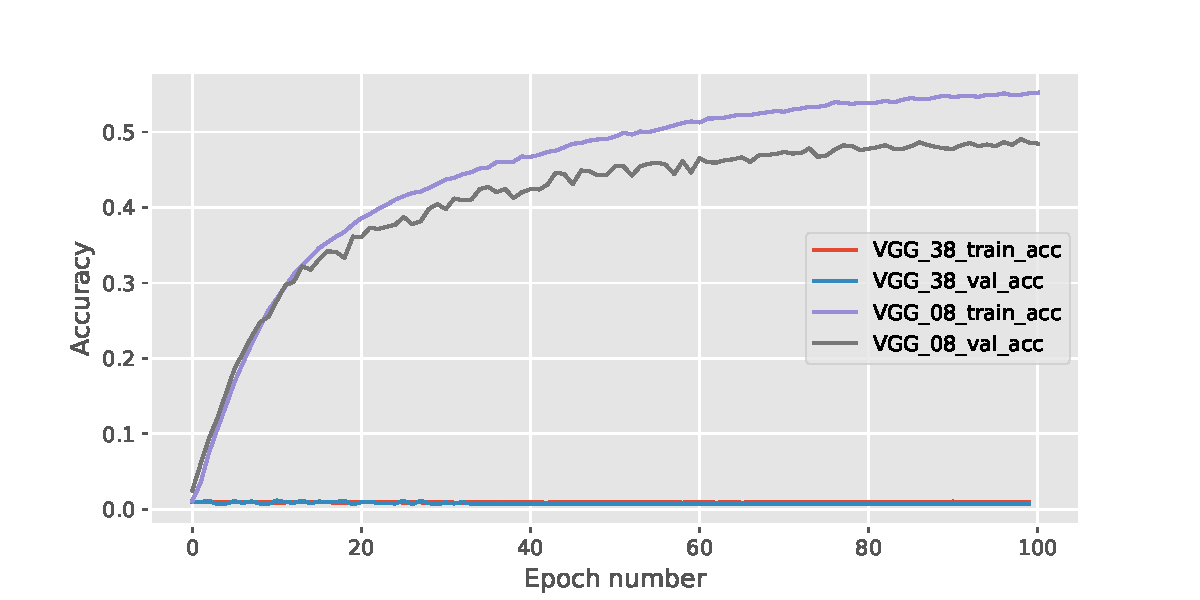
\includegraphics[width=\linewidth]{figures/accuracy_plot.pdf}
        \caption{Classification accuracy per epoch}
        \label{fig:acc_curves}
    \end{subfigure}
    \caption{Training curves for VGG08 and VGG38 in terms of (a) cross-entropy error and (b) classification accuracy}
    \label{fig:curves}
\end{figure}

\begin{figure}[t]
    \centering
    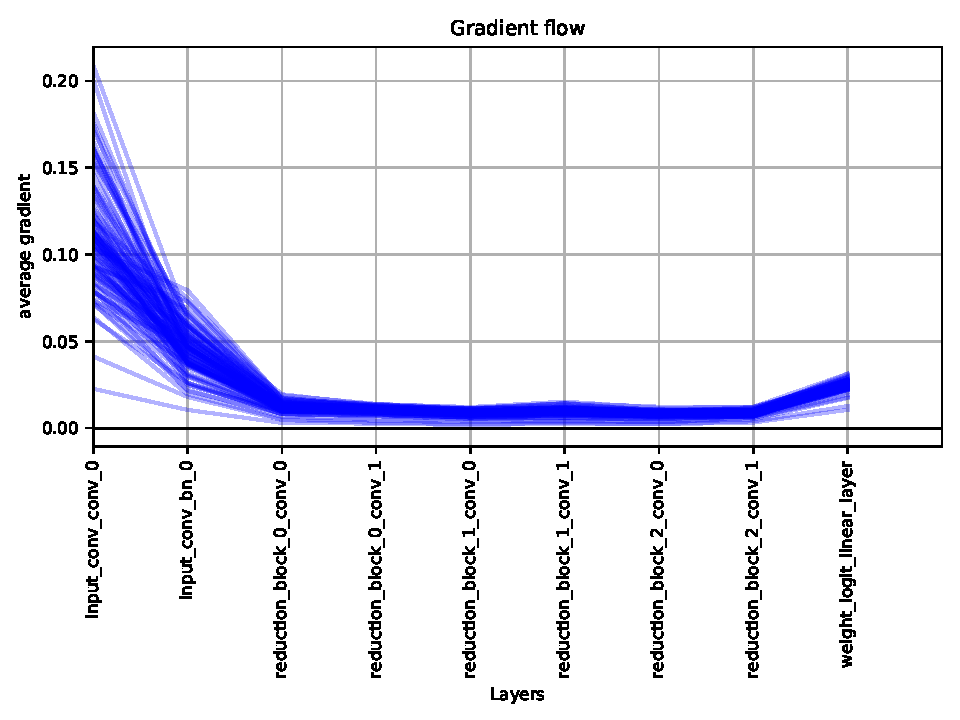
\includegraphics[width=\linewidth]{figures/grad_flow_vgg08.pdf}
    \caption{Gradient flow on VGG08}
    \label{fig:grad_flow_08}
\end{figure}

\questionFigureThree

Concretely, training deep neural networks typically involves three steps: forward
pass, backward pass (or backpropagation algorithm~\cite{rumelhart1986learning}) and weight update.
The first step involves passing the input $\bx^{(0)}$ to the network and producing 
the network prediction and also the error value.
In detail, each layer takes in the output of the previous layer and applies
a non-linear transformation:
\begin{equation}
\label{eq.fprop}
\bx^{(l)} = f^{(l)}(\bx^{(l-1)}; W^{(l)})    
\end{equation} 
where $(l)$ denotes the $l$-th layer in $L$ layer deep network,
$f^{(l)}(\cdot,W^{(l)})$ is a non-linear transformation for layer $l$, and $W^{(l)}$ are the weights of layer $l$.
For instance, $f^{(l)}$ is typically a convolution operation followed by an activation function in convolutional neural networks.
The second step involves the backpropagation algorithm, where we calculate the gradient of an error function $E$ (\textit{e.g.} cross-entropy) for each layer's weight as follows:

\begin{equation}
    \label{eq.bprop}
\frac{\partial E}{\partial W^{(l)}} = \frac{\partial E}{\partial \bx^{(L)}} \frac{\partial \bx^{(L)}}{\partial \bx^{(L-1)}} \dots \frac{\partial \bx^{(l+1)}}{\partial \bx^{(l)}}\frac{\partial \bx^{(l)}}{\partial W^{(l)}}.
\end{equation}

This step includes consecutive tensor multiplications between multiple
partial derivative terms.
The final step involves updating model weights by using the computed 
$\frac{\partial E}{\partial W^{(l)}}$ with an update rule.
The exact update rule depends on the optimizer.

A notorious problem for training deep neural networks is the vanishing/exploding gradient
problem~\cite{bengio1993problem} that typically occurs in the backpropagation step when some of partial gradient terms in Eq.~\ref{eq.bprop} includes values larger or smaller than 1.
In this case, due to the multiple consecutive multiplications, the gradients \textit{w.r.t.} weights can get exponentially very small (close to 0) or very large (close to infinity) and
prevent effective learning of network weights.


%


Figures~\ref{fig:grad_flow_08} and \ref{fig:avg_grad_flow_38} depict the gradient flows through VGG architectures \cite{simonyan2014very} with 8 and 38 layers respectively, trained and evaluated for a total of 100 epochs on the CIFAR100 dataset. \questionOne.


\section{Background Literature}
\label{sec:lit_rev}
In this section we will highlight some of the most influential
papers that have been central to overcoming the VGP in
deep CNNs.

\paragraph{Batch Normalization}\cite{ioffe2015batch}
BN seeks to solve the  problem of 
internal covariate shift (ICS), when distribution of each layer’s 
inputs changes during training, as the parameters of the previous layers change. 
The authors argue that without batch normalization, the distribution of
each layer’s inputs can vary significantly due to the  stochastic nature of randomly sampling mini-batches from your
training set. 
Layers in the network hence must continuously adapt to these high variance distributions which hinders the rate of convergence gradient-based optimizers.
This optimization problem is exacerbated further with network depth due
to the updating of parameters at layer $l$ being dependent on
the previous $l-1$ layers.

It is hence beneficial to embed the normalization of
training data into the network architecture after work from
LeCun \emph{et al.} showed that training converges faster with
this addition \cite{lecun2012efficient}. Through standardizing
the inputs to each layer, we take a step towards achieving
the fixed distributions of inputs that remove the ill effects
of ICS. Ioffe and Szegedy demonstrate the effectiveness of
their technique through training an ensemble of BN
networks which achieve an accuracy on the ImageNet classification
task exceeding that of humans in 14 times fewer
training steps than the state-of-the-art of the time.
It should be noted, however, that the exact reason for BN’s effectiveness is still not completely understood and it is 
an open research question~\cite{santurkar2018does}.



\paragraph{Residual networks (ResNet)}\cite{he2016deep} A well-known way of mitigating the VGP is proposed by He~\emph{et al.} in \cite{he2016deep}. In their paper, the authors depict the error curves of a 20 layer and a 56 layer network to motivate their method. Both training and testing error of the 56 layer network are significantly higher than of the shallower one.

\questionTwo.

Residual networks, colloquially
known as ResNets, aim to alleviate VGP through the
incorporation of skip connections that bypass the linear
transformations into the network architecture. 
The authors argue that this new mapping is significantly easier
to optimize since if an identity mapping were optimal, the
network could comfortably learn to push the residual to
zero rather than attempting to fit an identity mapping via
a stack of nonlinear layers. 
They bolster their argument
by successfully training ResNets with depths exceeding
1000 layers on the CIFAR10 dataset.
Prior to their work, training even a 100-layer was accepted
as a great challenge within the deep learning community.
The addition of skip connections solves the VGP through
enabling information to flow more freely throughout the
network architecture without the addition of neither extra
parameters, nor computational complexity.

\section{Solution overview}
\subsection{Batch normalization}





BN has been a standard component in the state-of-the-art 
convolutional neural networks \cite{he2016deep,huang2017densely}.
% As mentioned in Section~\ref{sec:lit_rev}, 
Concretely, BN is a
layer transformation that is performed to whiten the activations
originating from each layer. 
As computing full dataset statistics at each training iteration
would be computationally expensive, BN computes batch statistics
to approximate them. 
Given a minibatch of $B$ training samples and their feature maps
 $X = (\bx^1, \bx^2,\ldots , \bx^B)$ at an arbitrary layer where $X \in \mathbb{R}^{B\times H \times W \times C}$, $H, W$ are the height, width of the feature map and $C$ is the number of channels, the batch normalization first computes the following statistics:

\begin{align}
\label{eq.bnstats}
    \mu_c &= \frac{1}{BWH}  \sum_{n=1}^{B}\sum_{i,j=1}^{H,W} \bx_{cij}^{n}\\
    \sigma^2_c &= \frac{1}{BWH}
    \sum_{n=1}^{B}\sum_{i,j=1}^{H,W} (\bx_{cij}^{n} - \mu_{c})^2
\end{align} where $c$, $i$, $j$ denote the index values for $y$, $x$ and channel coordinates of feature maps, and $\bm{\mu}$ and $\bm{\sigma}^2$ are the mean and variance of the batch.

BN applies the following operation on each feature map in batch B for every $c,i,j$:
\begin{equation}
\label{eq.bnop}
\text{BN}(\bx_{cij}) = \frac{\bx_{cij} - \mu_{c}}{\sqrt{\sigma^2_{c}} + \epsilon} * \gamma_{c} + \beta_{c}
\end{equation} where $\gamma \in \mathbb{R}^C$ and $\beta\in \mathbb{R}^C$ are learnable parameters and $\epsilon$ is a small constant introduced to ensure numerical stability.

At inference time, using batch statistics is a poor choice as it introduces noise in the evaluation and might not even be well defined. Therefore, $\bm{\mu}$ and $\bm{\sigma}$ are replaced by running averages of the mean and variance computed during training, which is a better approximation of the full dataset statistics.

Recent work
has shown that BatchNorm has a more fundamental
benefit of smoothing the optimization landscape during
training \cite{santurkar2018does} thus enhancing the predictive
power of gradients as our guide to the global minimum.
Furthermore, a smoother optimization landscape should
additionally enable the use of a wider range of learning
rates and initialization schemes which is congruent with the
findings of Ioffe and Szegedy in the original BatchNorm
paper~\cite{ioffe2015batch}.


\subsection{Residual connections}

Residual connections are another approach used in the state-of-the-art Residual Networks~\cite{he2016deep} to tackle the vanishing gradient problem.
Introduced by He et. al.~\cite{he2016deep}, a residual block consists of a
convolution (or group of convolutions) layer, ``short-circuited'' with an identity mapping.
More precisely, given a mapping $F^{(b)}$ that denotes the transformation of the block $b$ (multiple consecutive layers), $F^{(b)}$ is applied to its input
feature map $\bx^{(b-1)}$ as $\bx^{(b)} = \bx^{(b-1)} + {F}(\bx^{(b-1)})$.

Intuitively, stacking residual blocks creates an architecture where inputs of each blocks
are given two paths : passing through the convolution or skipping to the next layer. A residual network can therefore be seen as an ensemble model averaging every sub-network
created by choosing one of the two paths. The skip connections allow gradients to flow
easily into early layers, since 
\begin{equation}
    \frac{\partial \bx^{(b)}}{\partial \bx^{(b-1)}} = \mathbbm{1} + \frac{\partial{F}(\bx^{(b-1)})}{\partial \bx^{(b-1)}}
    \label{eq.grad_skip}
\end{equation} where $\bx^{(b-1)} \in \mathbb{R}^{C \times H \times W }$ and $\mathbbm{1}$ is a $\mathbb{R}^{C \times H \times W}$-dimensional tensor with entries 1 where $C$, $H$ and $W$ denote the number of feature maps, its height and width respectively. 
Importantly, $\mathbbm{1}$ prevents the zero gradient flow.


\section{Experiment Setup}

\questionFigureFour

\questionFigureFive

\questionTableOne

We conduct our experiment on the CIFAR100 dataset \cite{krizhevsky2009learning},
which consists of 60,000 32x32 colour images from 100 different classes. The number of samples per class is balanced, and the
samples are split into training, validation, and test set while
maintaining balanced class proportions. In total, there are 47,500; 2,500; and 10,000 instances in the training, validation,
and test set, respectively. Moreover, we apply data augmentation strategies (cropping, horizontal flipping) to improve the generalization of the model.

With the goal of understanding whether BN or skip connections
help fighting vanishing gradients, we first test these
methods independently, before combining them in an attempt
to fully exploit the depth of the VGG38 model.

All experiments are conducted using the Adam optimizer with the default
learning rate (1e-3) -- unless otherwise specified, cosine annealing and a batch size of 100
for 100 epochs. 
Additionally, training images are augmented with random 
cropping and horizontal flipping.
Note that we do not use data augmentation at test time.
These hyperparameters along with the augmentation strategy are used
to produce the results shown in Fig.~\ref{fig:curves}.

When used, BN is applied
after each convolutional layer, before the Leaky
ReLU non-linearity. 
Similarly, the skip connections are applied from 
before the convolution layer to before the final activation function
of the block as per Fig.~2 of \cite{he2016deep}. 
Note that adding residual connections between the feature maps before and after downsampling requires special treatment, as there is a dimension mismatch between them. 
Therefore in the coursework, we do not use residual connections in the down-sampling blocks. However, please note that batch normalization should still be implemented for these blocks. 

\subsection{Residual Connections to Downsampling Layers}
\label{subsec:rescimp}

\questionThree.


\section{Results and Discussion}
\label{sec:disc}

\questionFour.

\section{Conclusion}
\label{sec:concl}

\questionFive.    

\bibliography{refs}

\end{document} 





